\documentclass[aspectratio=169]{beamer}

\usepackage{multirow}

\usetheme{vega}
\renewcommand{\textSupervisors}    {Supervisor}

\title{Forecasting the Yield Curve: An Econometric Study}
\subtitle{}
\author{Vsevolod Zaostrovsky, Ivan Cherepakhin, Artemy Sazonov}
\institute{Lomonosov Moscow State University}
\supervisor{Ivan P. Stankevich}

\begin{document}
\maketitle

\begin{frame}{YC and data}
    \begin{figure}
        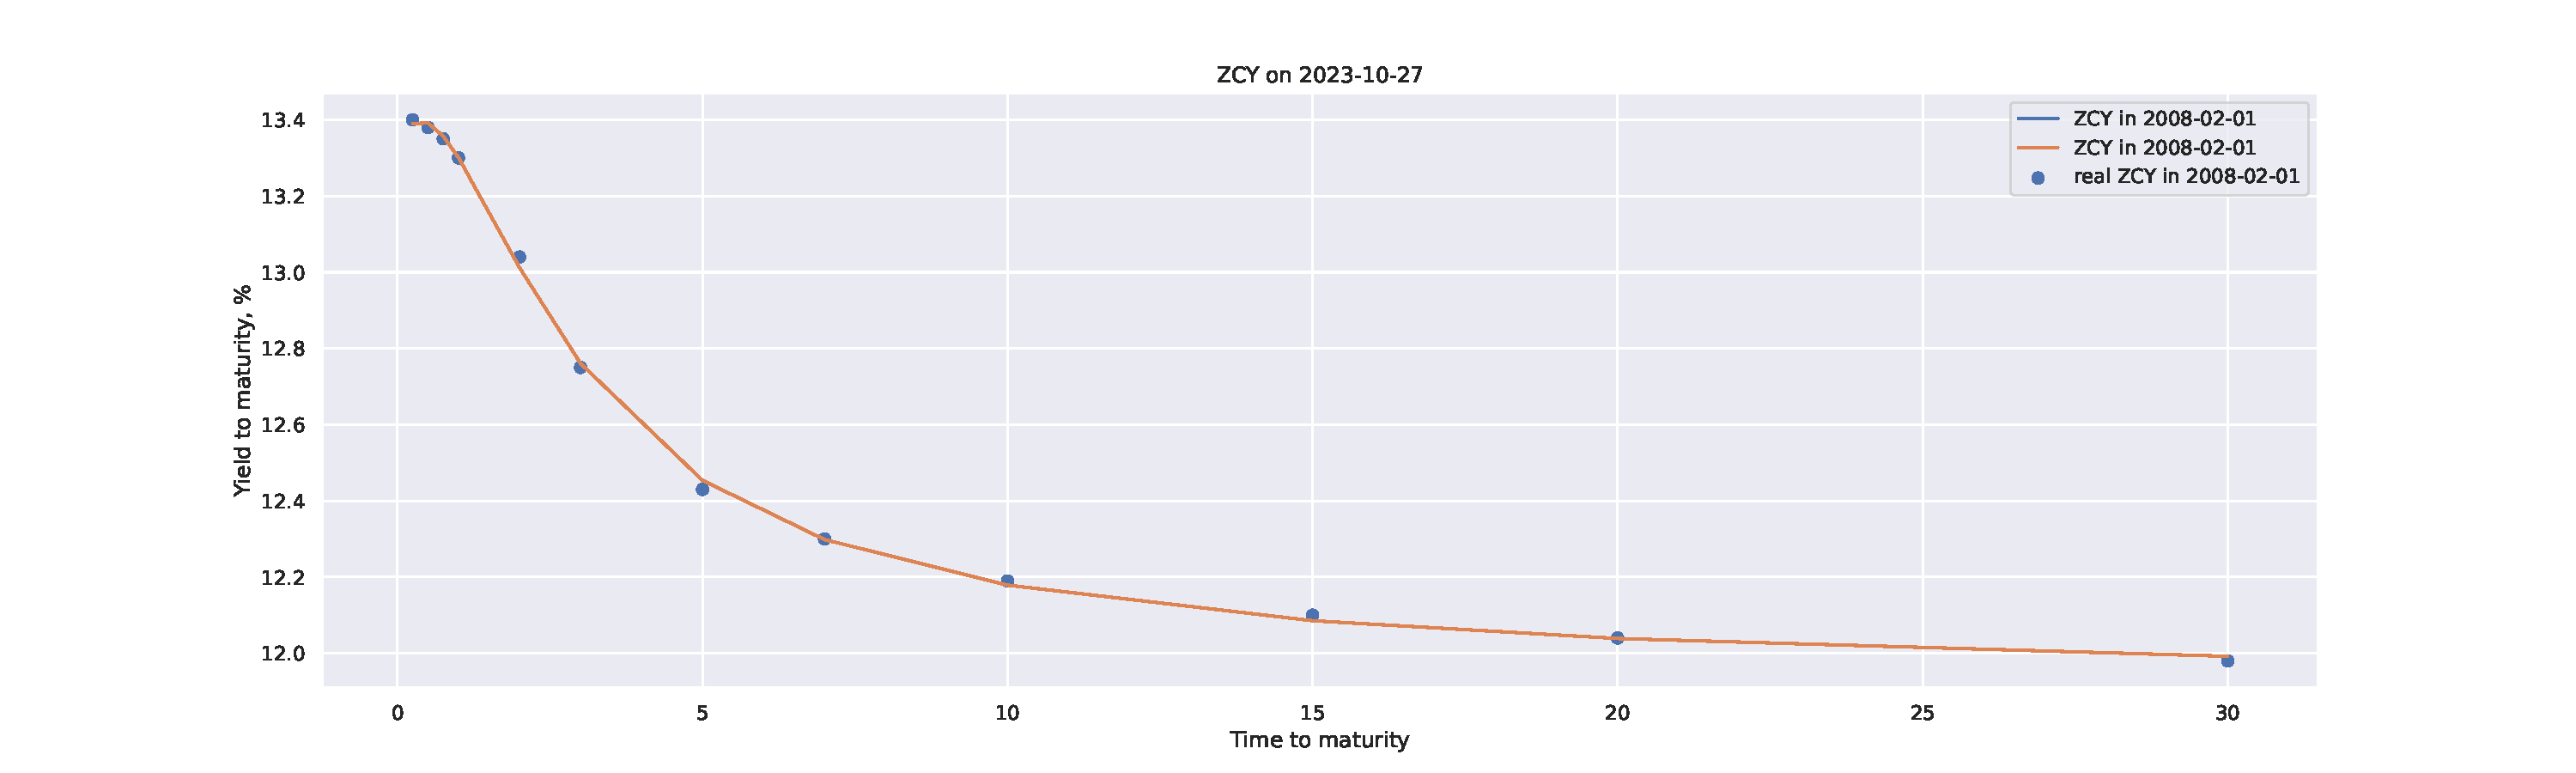
\includegraphics[scale=0.21]{fig/ZCYp.pdf}
        \caption{Yield Curve }
        \label{fig:YTMp}
    \end{figure}
    \begin{equation}\label{eq:NS}
        G(T) = \beta_0 + (\beta_1+\beta_2)\frac{\tau}{T}\left(1-e^{-\frac{T}{\tau}}\right)-\beta_2  e^{-\frac{T}{\tau}},
    \end{equation}
    where $T$ is the time to maturity, $G(T)$ is the yield estimator, 
    and the parameters to be estimated are: $\beta_0$ is the long-run of zero-bond yields, $\beta_1$ is the mid-run of zero-bond yields, 
    $\beta_2$ is the short-run of zero-bond yields.
    
\end{frame}

\begin{frame}{Structural breaks in factors}

    \begin{figure}
        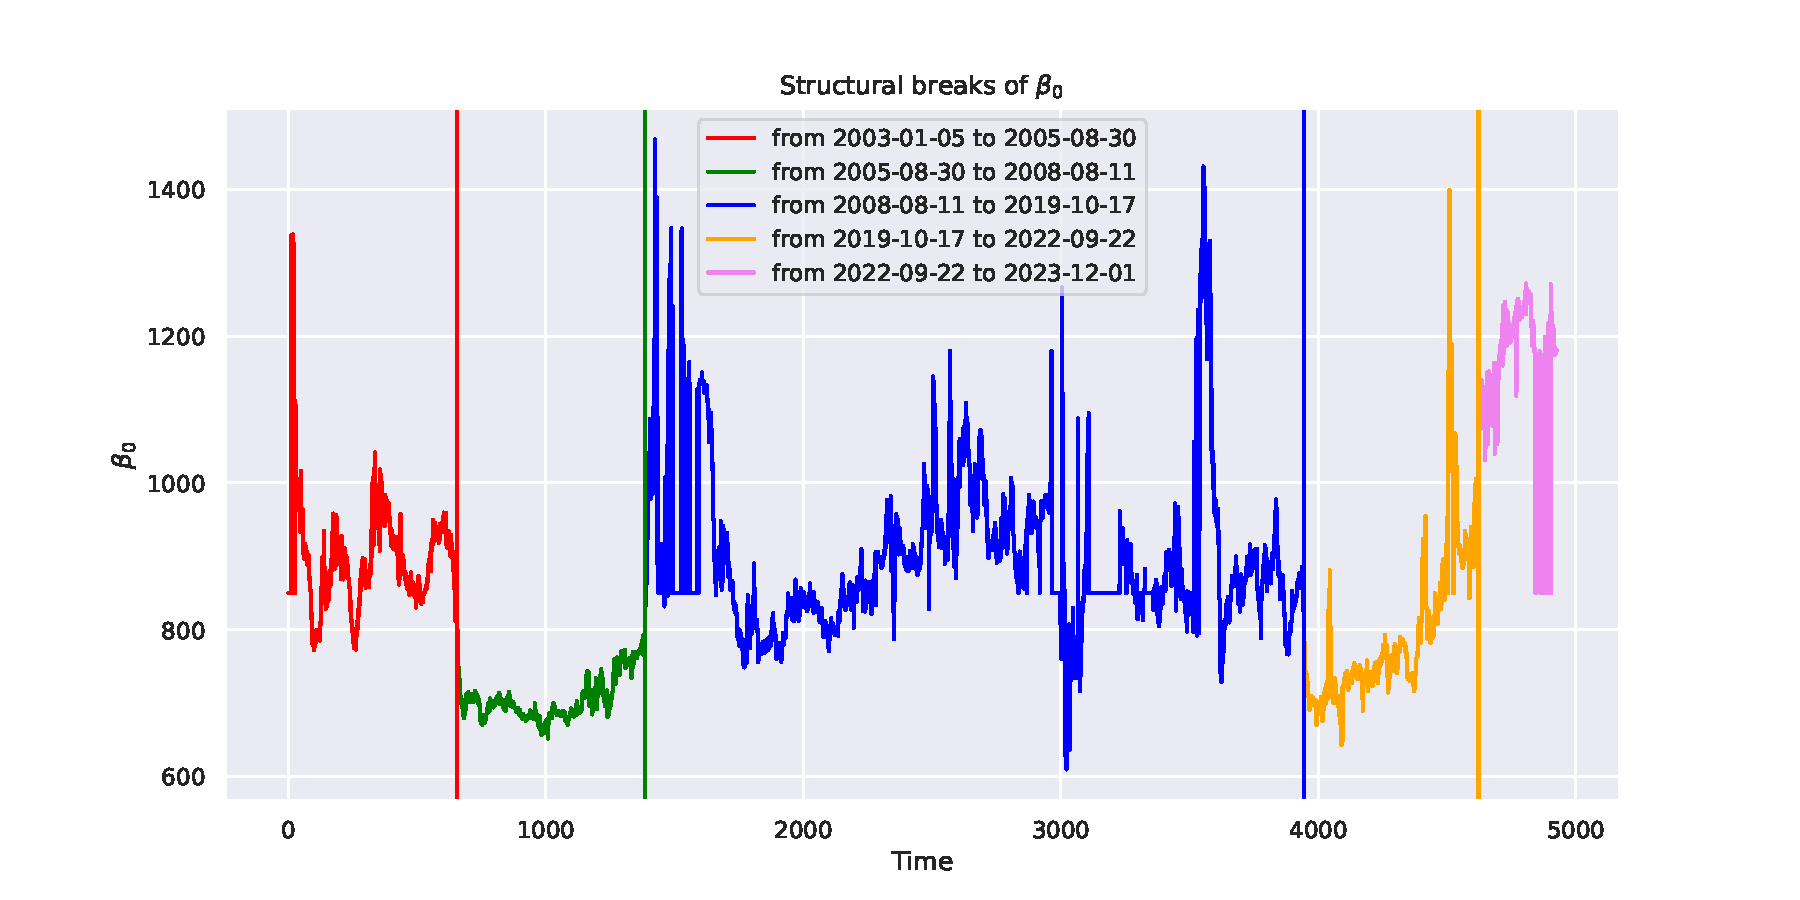
\includegraphics[scale=0.43]{fig/StrBreaks.pdf}
        \caption{Yield Curve }
        \label{fig:StrBreaks}
    \end{figure}
\end{frame}

\begin{frame}{Structural breaks in factors}
    \begin{enumerate}
        \item 2005: The complete stabilization of the Russian economy, the war in Iraq. 
        \item 2008: the Russo-Georgian Conflict and the beginning of the world finanical crisis.
        \item 2018: protests from March 2017 to the end of 2018. Also, it was a 2018 FIFA World Cup.
        \item 2020: COVID-19 pandemic.
        \item 2022: special military operation.
    \end{enumerate}

\end{frame}


    \begin{frame}{Structural breaks}
        \begin{table}[H]
        \begin{center}
            \begin{tabular}{|c|c|c|c|c|}
                \hline
            Factor    &  MAPE         & MAE         & RMSE          \\ \hline
            $\beta_0$ &  0.006        & 5.5102      & 6.0729        \\ \hline 
            $\beta_1$ &  0.3471       & 29.3697     & 32.2907       \\ \hline 
            $\beta_2$ &  0.5223       & 93.8611     & 95.6724       \\ \hline 
            $\tau$    &  0.9588       & 1.8988      & 1.987         \\ \hline
            \end{tabular}
        \end{center}
        \caption{NS factors forecasting results using ARIMA for the last segment.}
    \end{table} 
    \begin{table}[H]
        \begin{center}
            \begin{tabular}{|c|c|c|c|}
                \hline
            Factor    &  MAPE         & MAE         & RMSE          \\ \hline
    
            $\beta_0$ &  0.0139       & 12.8457     & 14.9255       \\ \hline 
            $\beta_1$ &  0.134        &  12.1766    &  15.9566      \\ \hline 
            $\beta_2$ &  0.3394       & 60.4861     &  61.5831      \\ \hline 
            $\tau$    &  0.3582       &  0.68       &  0.7972       \\ \hline
            \end{tabular}
            \caption{NS factors forecasting results using VAR for the last segment.}
        \end{center}
    \end{table} 



    \end{frame}

    \begin{frame}{Nelson-Siegel factors forcast using ARIMA}
        \begin{figure}
            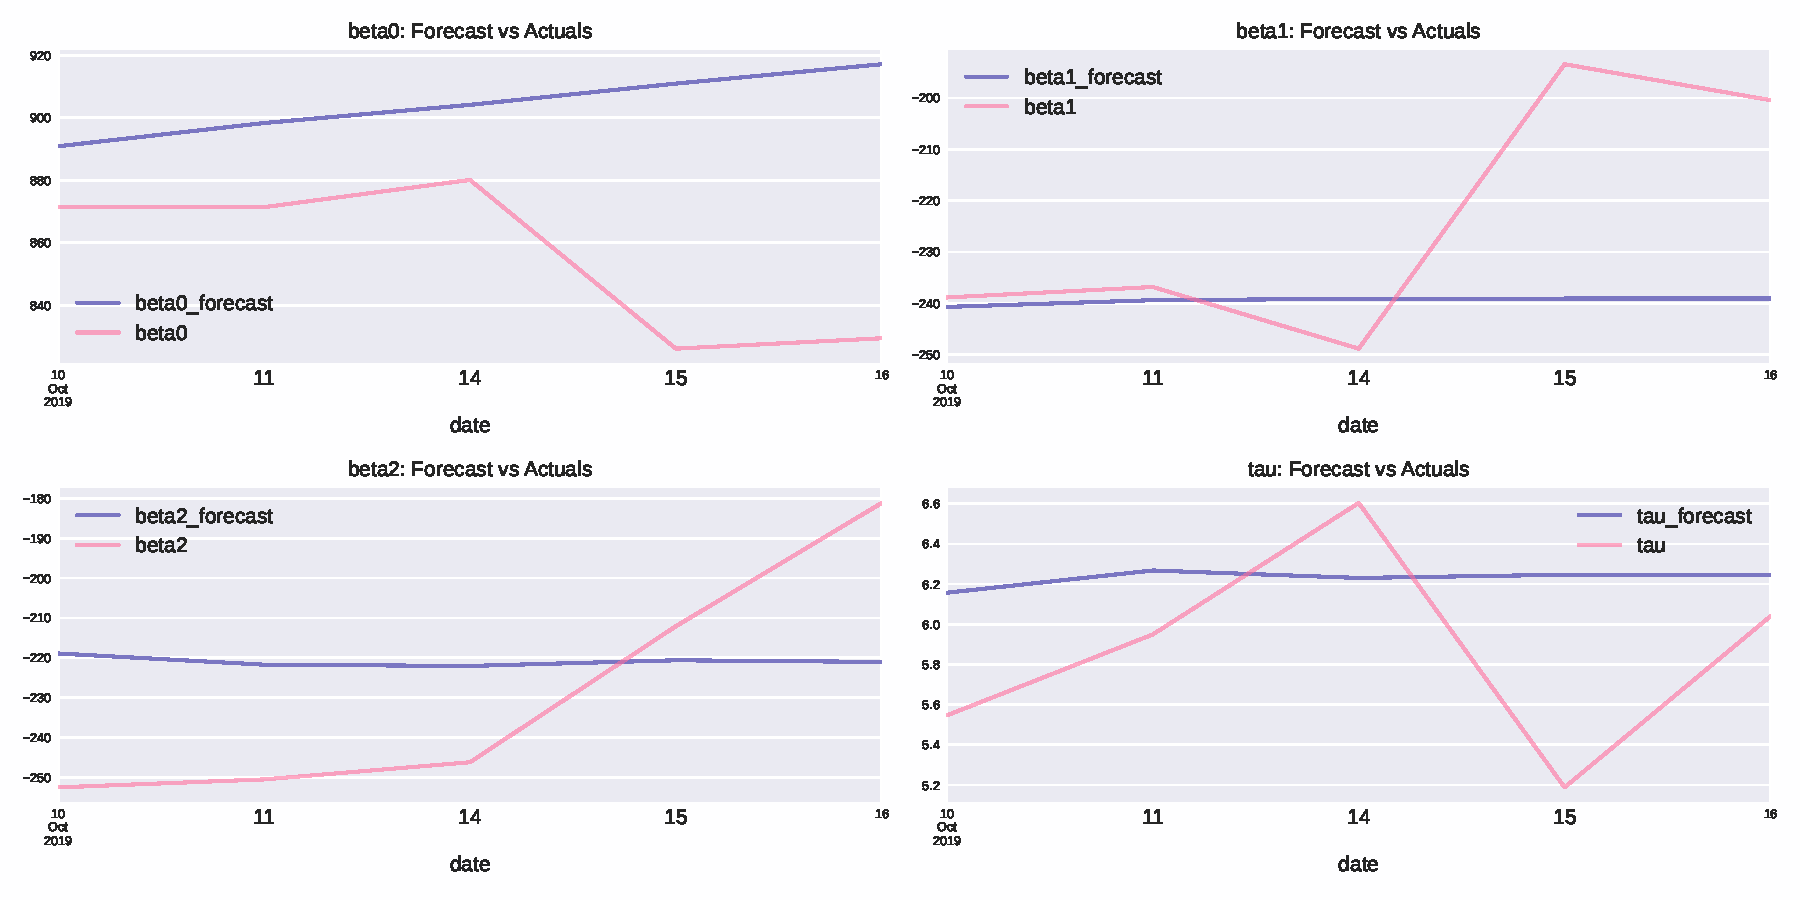
\includegraphics[scale=0.47]{fig/ARIMAfcst.pdf}
            \caption{Nelson-Siegel factors forcast using ARIMA}
            \label{fig:VARnsfcst}
        \end{figure}
    \end{frame}


    \begin{frame}{Nelson-Siegel factors forcast using VAR}
        \begin{figure}
            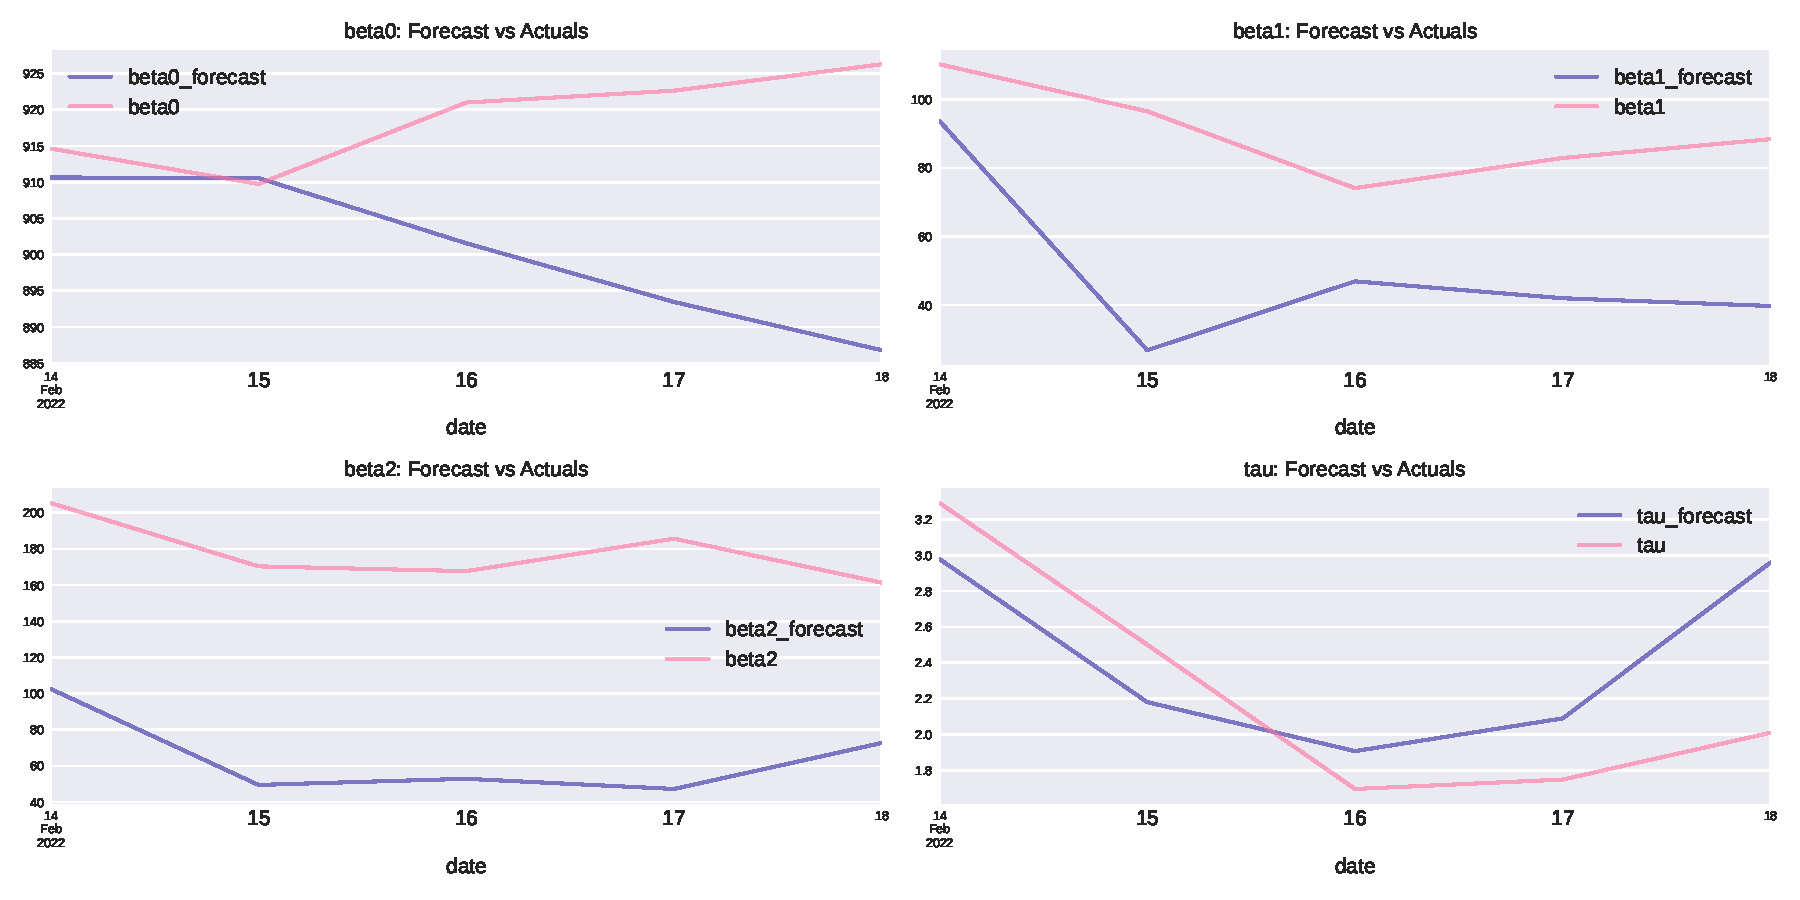
\includegraphics[scale=0.47]{fig/VARforcasts.pdf}
            \caption{Nelson-Siegel factors forcast using VAR}
            \label{fig:VARnsfcst}
        \end{figure}
    \end{frame}


\end{document}